\documentclass{article}
\usepackage[utf8]{inputenc}

\usepackage[margin=1in]{geometry} 
\usepackage{amsmath}
\usepackage{amssymb}
\usepackage{amsthm}
\usepackage{accents}
\usepackage{graphicx}
\graphicspath{{Images/}}


\setlength{\oddsidemargin}{0in}
\setlength{\textwidth}{6.5in}
\setlength{\topmargin}{-.55in}
\setlength{\textheight}{9in}
\pagestyle{empty}


\title{Problem Set 7 (Astrophysics)}
\author{Michael Nameika}
\date{April 2022}

\begin{document}

\maketitle

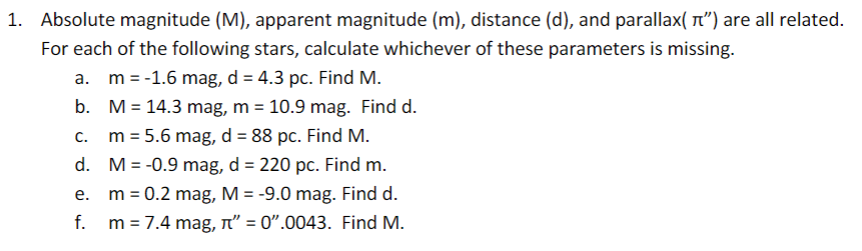
\includegraphics[scale = 0.8]{probset7prob1.PNG}

Recall the formula that relates absolute magnitude, apparent magnitude, and distance (in parsecs):
\begin{equation}
    M = m + 5 - 5\log_{10}{(d)}
\end{equation}

a) Plugging in the given values into equation (1), we find that
\[M = -1.6 + 5 - 5\log_{10}{(4.3)}\]
\[ \approx 0.233\]
So the absolute magnitude of a star with apparent magnitude of -1.6 at a distance of 4.3 $pc$ is approximately mag 0.233.

b) Plugging in the values into equation (1), we find that 
\[14.3 = 10.9 + 5 - 5\log_{10}{(d)}\]
and rearranging and solving for $d$, we get
\[d = 10^{1.6/5} \approx 2.09 \: pc\]
So the distance of a star with an absolute magnitude of 14.3 and apparent magnitude of 10.9 is approximately 2.09 $pc$.

c) Plugging in the given values into equation (1), we find that
\[M = 5.6 + 5 - 5\log_{10}{(88)}\]
\[ \approx 0.878\]
So the absolute magnitude of a star at a distance of 88 $pc$ and an apparent magnitude of 5.6 is approximately mag 0.878.

d) Plugging in the given values into equation (1) and solving for the apparent magnitude, we find that
\[m = -5.9 + 5\log_{10}{(220)}\]
\[\approx 5.81\]
So the apparent magnitude of a star at a distance of 220 $pc$ with an absolute magnitude of -0.9 is approximately 5.81.

e) Plugging in the given values into equation (1) and solving for $d$, we find
\[d = 10^{14.2/5}\]
\[\approx 691.8 \:pc\]
So the distance of a star with an apparent magnitude of 0.2 and an absolute magnitude of -9 is approximately 691.8 $pc$.

f) To begin, we must find the distance in parsecs by using the relationship
\[d = \frac{1}{\pi''}\]
Doing so, we find
\[d \approx 232.6 \:pc\]
And plugging this along with the other given values into equation (1), we find that 
\[M = 7.4 + 5 - 5\log_{10}{(232.6)}\]
\[\approx 0.567\]
So the absolute magnitude of a star with apparent magnitude of 7.4 at a distance of 232.6 $pc$ is approximately Mag 0.567.
\newline

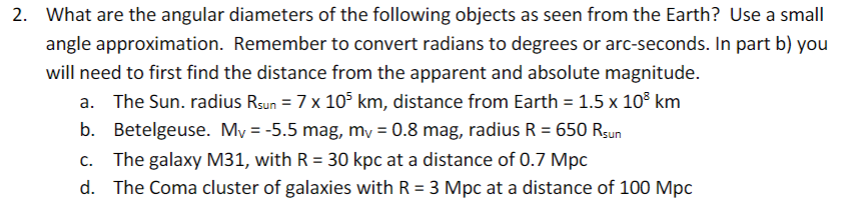
\includegraphics[scale = 0.8]{probset7prob2.PNG}

Notice from the diagram below that the angular size is given by $\tan{(\frac{\theta}{2})} = \frac{R}{2d}$ and using the small angle approximation, we find that $\theta \approx \frac{R}{d}$.
\begin{center}
    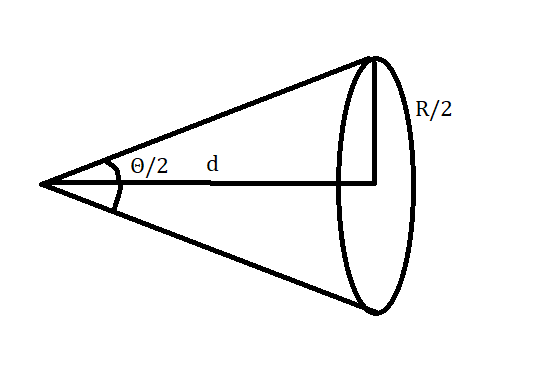
\includegraphics[scale = 0.8]{angular size.PNG}
\end{center}

a) Using the approximation we found above, and the data given, we find that
\[\theta_{Sun} \approx \frac{7 \times 10^5 \: km}{3 \times 10^8 \: km}\]
\[\approx 0.00233 \:rad\]
\[ = 0.27^{\circ}\]
So the angular diameter of the Sun as seen from Earth is approximately $0.27^{\circ}$.

b) To begin, we must figure out the distance to Betelgeuse. Using equation (1) we find that
\[d \approx 10^{11.3/5}\]
\[\approx 181.97 \:pc\]
\[\approx 5.615 \times 10^{15} \: km\]
then the angular diameter is 
\[\theta \approx \frac{650 \times 7 \times 10^5 \: km}{5.615 \times 10^{15} \:km}\]
\[\approx 8.10 \times 10^{-8} \: rad\]
\[\approx 0.017 \:\text{arcsec}\]
So the angular diameter of Betelgeuse as seen from the Earth is approximately 0.017 arcseconds.

c) Using the given data, we find that 
\[\theta \approx \frac{30 \: kpc}{700 \: kpc}\]
\[\approx 0.043 \:rad\]
\[\approx 2.46^{\circ}\]
So the Andromeda Galaxy has an angular diameter as seen from the Earth of approximately $2.46^{\circ}$.

d) Using the given data, we find that 
\[\theta \approx \frac{3 \:Mpc}{100 \: Mpc}\]
\[\approx 1.72^{\circ}\]
So the Coma Cluster has an angular diameter as seen from the Earth of approximately $1.72^{\circ}$.
\newline

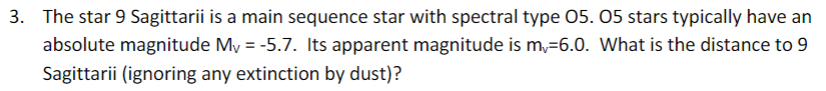
\includegraphics[scale = 0.8]{probset7prob3.PNG}

Using equation (1), we find that
\[d = 10^{16.7/5}\]
\[\approx 2187.76 \:pc\]
So the distance to 9 Sagittarii is approximately 2187.76 $pc$. (9 Sagittarii is the brightest star seen imposed on M8, the Lagoon nebula, a nice summertime object that is visible to the naked eye in many dark sky locations.)
\newline

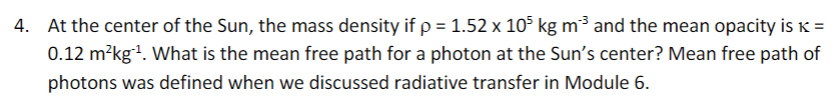
\includegraphics[scale = 0.8]{probset7prob4.PNG}

The equation for the mean free path of a photon given density and opacity is given by
\begin{equation}
    mfp = \frac{1}{\rho \kappa}
\end{equation}
Plugging in the given values into equation (2), we find 
\[mfp = \frac{1}{(1.52 \times 10^{5} \:kg m^{-3})(0.12 \:m^2 kg^{-1})}\]
\[\approx 5.48 \times 10^{-5} \:m\]
So the mean free path for a photon at the center of the Sun is approximately $5.48 \times 10^{-5} \:m$.
\newline

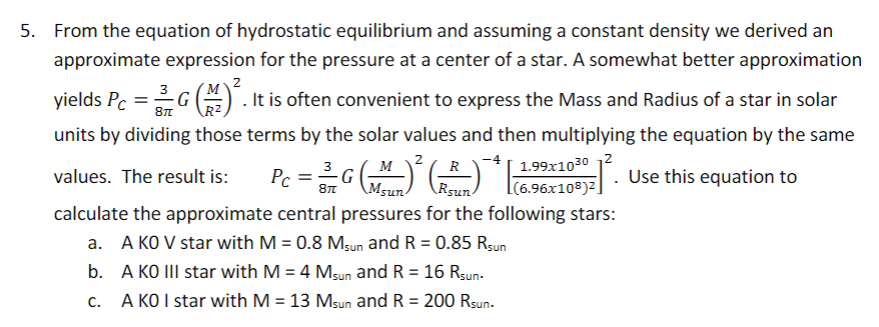
\includegraphics[scale = 0.8]{probset7prob5.PNG}
\begin{equation}
    P_C = \frac{3}{8\pi}G\left(\frac{M}{M_{Sun}}\right)^2\left(\frac{R}{R_{Sun}}\right)^{-4}\left[\frac{1.99 \times 10^{30}}{(6.96 \times 10^8)^2}\right]^2
\end{equation}

a) Using the given data and plugging it into equation (3), we find
\[P_{C_{K0\:V}} = \frac{3}{8\pi}G\left(\frac{0.8 \:M_{Sun}}{M_{Sun}}\right)^2\left(\frac{0.85 \:R_{Sun}}{R_{Sun}}\right)^{-4}\left[\frac{1.99 \times 10^{30}}{(6.96 \times 10^8)^2}\right]^2\]
\[\approx 1.65 \times 10^{14} \: Pa\]

b) Using the given data and plugging it into equation (3), we find
\[P_{C_{K0\:III}} = \frac{3}{8\pi}G\left(\frac{4 \:M_{Sun}}{M_{Sun}}\right)^2\left(\frac{16 \:R_{Sun}}{R_{Sun}}\right)^{-4}\left[\frac{1.99 \times 10^{30}}{(6.96 \times 10^8)^2}\right]^2\]
\[\approx 3.280 \times 10^{10} \: Pa\]


c) Using the given data and plugging it into equation (3), we find
\[P_{C_{K0\:I}} = \frac{3}{8\pi}G\left(\frac{13 \:M_{Sun}}{M_{Sun}}\right)^2\left(\frac{200 \:R_{Sun}}{R_{Sun}}\right)^{-4}\left[\frac{1.99 \times 10^{30}}{(6.96 \times 10^8)^2}\right]^2\]
\[\approx 1.42 \times 10^{7} \: Pa\]
\end{document}
